\chapter{Routes to Enlightenment!}

Those of us who chose TIFR were taken to visit the experi\-mental 
laboratories in TIFR. I found that all the laboratories were stack\-ed 
with huge electronic boxes. Those days all electronic instruments used 
thermionic valves and hence were very big. I was thoroughly discouraged. 
I had a dread of electronics since my bad experience in MCC. So although 
I liked experimental physics, I had to do theoretical physics.

%~ \vspace{-\topsep}

\vspace{-.3cm}

\section*{Tata Institute of Fundamental Research I\\ (1958 to 1961)}

\vspace{-.2cm}

But for theoretical physics also I had a problem. Theory needs maths in 
which I was poor. So when I went to see KS Singhvi, the head of the 
theory group, I told him that I wanted to do theoreti\-cal physics, but I 
am not sure since I was not good in maths. He said he does not know any 
mathematics! So I joined Theory.

A few trainees who joined Theory group in the early years were Sudhanshu 
Jha and K V L Sarma both from the first batch and Mukunda and Divakaran 
from the second batch. The atmosphere for study was very good and there 
was hardly any restriction on what we can do. There were occasional 
lectures and seminars which we attended.

Since my mind was bent on understanding physics at its most fundamental 
level, I first took up the study of Quantum Mecha\-nics, since my 
knowledge of it was not strong. For any question that I asked, the 
answer was in Quantum Mechanics. I sat with L I Schiff's book for many 
months and mastered it. The other books I liked were PAM Dirac, the 
Bible of QM, Pauling and Wilson, an easy-to-understand book and Heitler, 
a very beautiful tiny book.

Then I turned to Nuclear Physics since that was the most fundamen\-tal 
subject at that time. I read Bethe and Morrison and then Blatt and 
Weisskopf. Went to Kailash Kumar and George Abraham for guidance. The 
former put me in contact with many body theory and the latter in contact 
with few body problems. Abraham even suggested a specific problem. He 
asked me to redo the deuteron and triton structure using the recently 
disco\-vered hard-core repulsion between nucleons.

I was not satisfied. I realized that the force between the nucleons 
comes from a deeper layer of reality which can be understood only from 
the then-new area called particle physics. There was no particle physics 
research in TIFR at that time. B M Udgaonkar (BMU) started studying 
hypernuclei which was in between nuclear and particle physics. 
Hypernuclei are nuclei in which one nucleon is replaced by a lambda 
particle. He introduced me to this subject and also to a few excellent 
reviews by Enrico Fermi on quantum theory of radiation and isospin 
symmetry.
 
He introduced me to Isospin and I calculated the ratio of Lambda going 
to $p + pi^-$ and $n + pi^0$ by using spurion technique. I thought it was a 
new result that I derived, but of course it was already well-known.

Udgaonkar was an excellent teacher. He had taught our ba\-tch of trainees 
reactor physics and the second batch quantum mechanics. Bhabha had sent 
him to France to learn about reactors, but BMU shifted to particle 
physics after returning.
\vskip 1pt
Soon SN Biswas and LK Pandit joined and real particle physics started in 
the Theory Group. I started reading particle physics and learnt that the 
real theory of particle physics was Quantum Field Theory (QFT). So 
finally I reached the destination of my ``Inward Bound" journey.

\newpage

I took up Bethe and Schweber's QFT and Jauch and Rohrlich's Theory of 
Photons and Electrons. I really loved the systematic treatment of QFT in 
Wentzel's book. I took it during my vacation in Kamuthi and read it even 
during the long train journeys.

My learning of QFT was systematized and consolidated only after I 
listened to LK Pandit's course of lectures on QFT. I was so impressed by 
his excellent lectures that I felt I achieved ``Enlightenment". I still 
remember lecturing to my friend Sudha\-nshu Jha on QFT during one of our 
evening walks along marine drive describing how I achieved my 
enlightenment. Maybe he was bored!
 
Soon I began to interact with Biswas and listened to his exce\-llent 
lectures on integral equations. I was very impressed that an integral 
equation can be easily solved if the kernel is separable. Combining my 
knowledge of hypernuclei learnt from R H Dalitz's papers with a 
separable kernel as the potential between lambda and nucleon was very 
easy thing to do, with Biswas's guidance. Thus was born my first 
research paper and we proved Gell-Mann's Global Symmetry which simply 
equated all the eight meson-baryon coupling constants did not work.

Dallaporta visited TIFR and gave a series of lectures on the Symmetries 
of Hadrons. This was in 1960 before SU(3) came and he mainly talked 
about Gell-Mann's Global Symmetry. Gell-mann came to the correct SU(3) 
symmetry in 1961 only after many wrong attempts! Mukunda and myself took 
notes of Dalla\-porta's lectures that came out as a TIFR yellow report.

Heitler came and lectured on nonlocal QFT. Divakaran and myself took 
notes and brought it out as another TIFR report.

Gyan Mohan gave a beautiful series of lectures on QFT in Heisenberg 
picture and the LSZ form of the S matrix.
\vskip 1pt
We were living in the servants' quarters attached to the Old Yacht Club 
where TIFR and AEET were situated, near Gate Way of India. This was the 
hostel of TIFR! One morning when I woke up, I was horrified to find that 
my finger-tips were of flesh colour. Mice had nibbled at them and 
removed flesh. They had done so with so much care that I was not 
awakened!

Bhabha had appointed an ex-ICS officer Mr EC Allardice, a Scotchman, 
as the Deputy Director (Administration) of TIFR. Se\-minar notices were 
put on the notice boards only after he approved them. Once a notice 
about a seminar on ``Odd-odd nuclei" was sent to him. Odd-odd, even-even, 
even-odd are technical terms in Nuclear Physics.\ Allardice said ``These 
Indians! tunda-tunda pani, garam-garam chai". So saying, he cut off one 
``odd" from ``Odd-odd" and sent it for the notice board!

I went on trekking in the western ghats with my friends who were senior 
to me: C S Warke, Biswarup Banerjee and K K Gupta. Once we were on a 
hill and I could see a long thing in a far-away hill moving. Obviously 
it was such a huge python which was visi\-ble from the next mountain!
 
On one such trip a funny thing happened. It was getting late and we 
wanted to take a short cut. One of us (KKG) suggested that we could cut 
the distance if we go through a railway tunnel. We were inside and it 
was dark. Suddenly we saw some light in the distance and we were happy 
that we were near the end of the tunnel. But the light grew bigger and 
bigger and we realized it was an approaching train! We were mortally 
afraid. It was a very narrow tunnel. There was space only for the 
railway track. All of us quickly hugged the tunnel wall. After the train 
passed, we thanked our stars and returned home, covered by soot and 
dust.

In those days, I used to see many films, sometimes more than one in a 
single day. English, Tamil, Hindi, even Marathi films! Those were really 
care-free days. There were two friends who were my constant companions. 
One was KG Nair a first batch trainee who intruduced me to the pleasures 
of PG Wodehouse. The other was VS Arunachalam who later rose very high 
in the DAE hierarchy.

There was an euphoria in the air. Remember only a decade had passed since Independence and there was an expectation of great things. I felt ``Nehru was in Delhi and Bhabha was in Bombay And all was well with our world".\ So my life and research would have gone on happily, but that was not to be.

One day Biswas told me that I must go to USA for PhD. I did not want to 
go; I did not think PhD was necessary for research. Those days PhD was 
a rarity. In MCC. Dr MA Thangaraj had great respect because of his 
doctorate degree, but most faculty members did not possess PhD degree. 
Also BMU in TIFR was not a PhD. But Biswas said that it was the policy 
of the Theory group to send young people for PhD. Biswas suggested that 
I should go to Maryland University. He liked Maryland University because 
JS Toll who had written some good papers on Dispersion Relations was 
there. He got the application form from Maryland. I was about to fill it 
when he came and said MGK Menon wanted to see me.

I went and saw him. He asked me why do I want to go to Maryland? I said 
I did not want to go, but Biswas asked me to go. He said I must go to 
Chicago University. He got the application form from Chicago and I 
filled it. Soon R H Dalitz was to visit TIFR and it was arranged that I 
must go to Chicago and work with Dalitz. TIFR packed me up and sent me! 
They bought the tickets, got the passport and visa.

Before that, I must describe what I call ``The Bangalore Eve\-nt". In the 
summer of 1961, the Summer School of TIFR was held at the campus of 
Indian Institute of Science, Bangalore. Gell-Mann and Dalitz were the 
lecturers and the audience consisted of students like me and many 
stalwarts like Homi Bhabha, MGK Menon, SN Biswas, LK Pandit, Virendra 
Gupta, Yash Pal and Alla\-di Ramakrishnan.

Gell-Mann lectured on his Eightfold Way version of Sakata's SU(3) 
theory, fresh from the anvil, even before publication. In Gell-Mann's 
Eightfold Way, proton, neutron and lambda were no longer a triplet, but 
a part of an octet.
 
During one of the lectures Dalitz asked him why was he igno\-ring the 
triplet which was needed to define the SU(3) symmetry. Gell-Mann evaded 
a direct answer in spite of Dalitz's repeated questioning.

\begin{figure}[h]
\centering
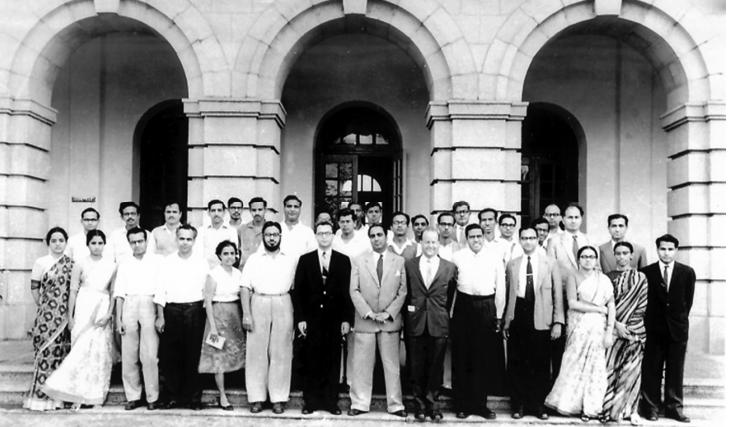
\includegraphics[width=\textwidth]{images/Rajaji-gellmann.jpg}
\caption{\small{Bangalore Summer School 1961 L to R: First row: Thunga (Alladi's student), Indumathi (Alladi's student), V Gupta, Yash Pal, Kharas (MGKM's secretary), MGK Menon, Gell-Mann, Bhabha, Dalitz, Alladi, Jallihal (Administrator), Radha (Alladi's student), Bhamathi, KK Gupta Second row: AP Balachandran, G Ramachandran, PP Divakaran (behind MGKM), GR (behind Bhabha), SN Biswas and LK Pandit (both between Alladi and Jallihal)}.}
\end{figure}
 
If Gell-Mann had answered Dalitz's question, quarks would have been born 
there in Bangalore, instead of having to wait for another three years. 
If any of us had answered the question, that would have been a major 
Indian discovery. This was a missed opportunity.

I sailed from Bombay to Liverpool in UK in August 1961 and flew from 
London to Chicago. The ship journey in SS Caledonia of Anchor Lines took 
about two weeks stopping at Karachi, Port Sudan and then at Alexandria 
in the Suez Canal. We were allo\-wed to land at all the ports and go into 
the city. At Port Sudan a few of us went to see a Hindi movie. On the 
way we met a Sudanese and asked him about the way to the theater. He 
looked at us, asked whether we are Indians. We said yes and he replied 
that he will not help us! While the ship was passing through the Suez 
Canal we made an in-land journey to Cairo and had a sight-seeing tour of 
the pyramids and the famous Cairo Museum.

I had planned to write the Candidacy Examination once I reached Chicago. 
So I spent the time in the ship preparing for that. I could revise 
whatever I knew in physics using the exce\-llent book by Kompaneets which 
presented all of Physics in a capsule form.
%~ \vspace{-\topsep}

\vspace{-.5cm}

\section*{University of Chicago (1961 to 1963)}
%~ \vskip -11pt

\vspace{-.2cm}

On the first day at Chicago University I had a pleasant experience. I 
came out of the International House where I was staying and asked a 
gentleman about the direction to the place where the inaugural meeting 
for beginners was to be held. He said he was also going there. We walked 
together. Imagine my surprise that he went to the stage to preside over 
the meeting! He was Beadle, a Nobel-Prize winner in biology and the 
President of the University.
    
Soon I wrote the dreaded Candidacy Exam and passed. It was considered a 
tough exam and some of the questions were the ones set by Enrico Fermi. 
Generally students took one year to clear it. But I was not a beginner 
since I had spent four years in TIFR. I was admitted into the PhD 
programme and I was also Research Assistant to Prof Dalitz. Apart from 
Dalitz, there were many luminaries - Nambu, Oehme, Sakurai, Telegdi, 
Wentzel and Chandrasekhar. I attended the lectures by all of them.

I was staying at the International House and once I was returning after 
midnight after completing the experiment which everybody had to do in 
the course, I was accosted by a group of black boys who asked for money. 
Fortunately I had some money in my pocket. I threw it at them and ran 
for my life.

Another time a group of us went to a Cinema Theater beyond the Midway 
and we were surrounded by hoodlums again. We ran into a Department 
store.


Such events were common those days in the area where the University was 
situated. I hear things are much better nowadays.

Since I was a vegetarian, I suffered. Those days it was very difficult 
to get veg food in USA. At the International house the only veg food was 
half-boiled rice and half-boiled cabbage. Ea\-ting that day after day, I 
got sick of it. What saved me was the pizza. Once I discovered that, 
everyday evening I phoned Nicky's Pizzeria and ordered for pizza. From 
that time, pizza has remained my favourite food!
 
One day, when I was coming out of the library in the physics department, 
I saw Chandrasekhar emerging from the office. I realized that I was 
lucky to be in Chicago University. When I learnt that he was giving 
courses in General Theory of Relativity (GRT) and later, on Mathematical 
Physics, I took both courses. At the beginning of the GRT course, he 
said that he was tea\-ching GRT since he wanted to learn it. He was 
absolutely right. Until then he had not worked in GRT. A few years after 
that he had mastered the subject and wrote his masterpiece ``GRT and 
Black Holes". His Mathematical Physics Course was on generali\-zed 
functions which he wanted to master and used it in studying Black Holes.
\vskip 1pt
Although I had attended two courses of Chandrasekhar, I hardly 
interacted with him. Chicago University had many Indian students. He had 
not interacted with any of them, as far I knew. Basically, he was a shy 
person. So imagine my surprise when one day, we got a letter from him 
inviting three of us A P Bala\-chandran who had completed his PhD in 
Madras and came to Chicago as a post-doc of Dalitz, R Ramachandran, a PhD student and myself. He sent detailed instructions on the train that we 
must take to go from Chicago to Yerkes, some 70 km away. He had 
positions at Chicago University and Yerkes Observatory.

\begin{figure}[H]
\centering
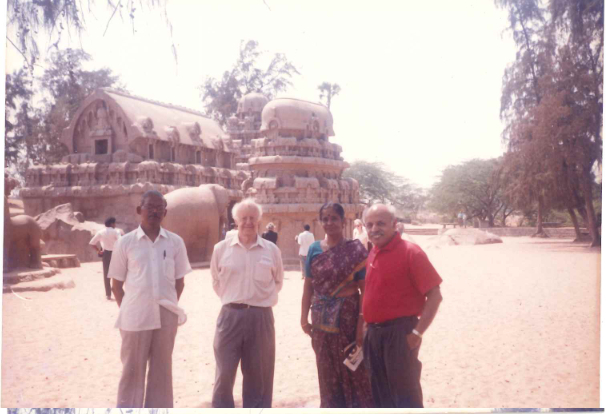
\includegraphics[width=0.9\textwidth]{images/new-images/07-Rajaji-Dalitz.jpg}
\caption{\small{With my thesis advisor Richard Dalitz in Mamalla\-puram when he visited Madras. Suthanthra and Ramachandran are also seen.}}
\end{figure}
\vspace{-\topsep}
He came to receive us at Yerkes railway station and took us to his home. 
His wife Lalitha cooked a tasty South Indian meal for us. He took us 
around to see the telescope. We then played some ball game in his garden 
while he took rest. After a while tea was ready and we watched the TV. 
On that day Edward Teller was giving evidence in front of a Government 
Committee about the H-bomb programme of the Soviet Union. He became 
emotional and we could see tears from his eyes. Chandra talked to us 
about Teller. Then the conversation shifted towards other to\-pics like 
particle physics, the subject of three of us and the science situation 
in India in which Chandra was greatly intere\-sted. We returned to Chicago 
with the satisfaction of spending a whole day in the company of a great 
man.

  
I take pride in the fact that I taught AK Ramanujam who later became
a famous Kannada poet and translated Sangam Tamil poetry, some Tamil.
At that time he was working as a research associate in the Department
of South Asian Studies in the Chica\-go University. He felt that the
Tamil I spoke was closer to the old Tamil since I come from the
southern part of Tamil Nadu. He asked me to speak Tamil and recorded it.
He paid me by the hour!


Dalitz asked me to make some calculations on hyper-nuclear physics. 
Although most of the main work was done by him, he included my name as a 
coauthor in the two published papers. I told him that I would like to 
work on a core topic of Particle Physics. He agreed.


At that time the dominant school of thought was the S matrix philosophy 
of GF Chew. Proving Mandelstam's double dispersion relations was 
considered the biggest challenge. Reinhard Oehme lectured to us on the 
many-sheeted S matrix, 


AP Balachandran who had already obtained his PhD in Mad\-ras and joined as 
Dalitz's post-doc was frightening students like me by talking about the 
theory of many complex variables and ``The Edge of the Wedge Theorem". He 
was very mathemati\-cally orien\-ted.


Those days you either group or disperse. The former led to SU(3) group 
and the later led to Dispersion Relations. An intere\-sting story about 
the proof of Dispersion Relations from Field Theory is the following:

\vspace{-\topsep}
\begin{itemize}
\itemsep=0pt
\item Feynman: What is Dispersion Relation? 
\item Wigner: What is Field Theory? 
\item Chew: What is Proof?
\end{itemize}
\vspace{-\topsep}

Dalitz showed me a preprint by Oakes and Yang who criticized the SU(3) 
work of Gell-Mann and Neeman on two counts:

\begin{enumerate}
\itemsep=0pt
\item The decimet baryons Delta (1238), Sigma (1320), Cascade (1520) and 
Omega minus (1672) occur as poles of the S matrix on different Riemann 
sheets and so, no smooth movement of them is possible to give a single 
pole in the exact SU(3) limit.

\item The mass-differences in the octet and decimet of particles are so 
large that no perturbative treatment is possible for the 
symmetry-breaking interaction to yield the Gell-Mann - Okubo mass 
formulae for their masses.
\end{enumerate}
\vspace{-\topsep}
I could immediately solve the first problem since I was already familiar 
with the different Riemann sheets of the S matrix, thro\-ugh the study of 
Oehme's papers. Solution was that there is a retinue of poles in 
different Riemann sheets corresponding to a single hadron. This was the 
discovery of what are now called ``Shadow Poles".

But instead of sending off our result to Physical Review Le\-tters as any 
American physicist would do, the conservative Dalitz sent a letter to 
Oakes and Yang. And Dalitz followed by me went away to Oxford. Meanwhile 
a host of other authors published the discovery of shadow poles. Dalitz 
and myself wrote up the result and published it in Physics Letters B 
later.

The second problem of Oakes and Yang did not have such a simple 
solution. It required detailed calculations based on mode\-ls and that 
formed the core of my PhD thesis.

%~ \vspace{-\topsep}

\vspace{-.3cm}

\section*{Oxford University (1963 to 1964)}

\vspace{-.2cm}


%~ \vskip -10pt

Dalitz decided to shift to Oxford University in 1963. Since my thesis 
work was almost complete, he gave me the choice of conti\-nuing at Chicago 
as his student or go to Oxford. I preferred the second choice and left 
Chicago.

I sailed from New York to London by the famous Queen Mary and completed 
the writing of my thesis in Oxford in 1964. Dalitz suggested that I must 
do post-doctoral work in some University in the USA, but I felt I must go 
back to TIFR since TIFR had sent me only for Ph D! So in the summer of 
1964 I sailed from Marseilles to Bombay by SS Vietnam, a French ship.

I must describe the three types of ships in which I have trave\-led. 
Since TIFR paid for my journey from Bombay, I traveled in a first class 
ship SS Caledonia. There were no classes and everybody was treated as a 
first class passenger. In fact the captain dined with us. There were many 
interesting games in which I participated and even won a prize (Nehru's 
``Discovery of India")! Although Queen Mary was a famous ship, Dalitz's 
research funds could pay only for a second class ticket, myself being a 
student. The third journey from Marseilles to Bombay was paid from my 
pocket and so it was a French ship SS Vietnam used to carry Vietnamese 
prisoners of war! But there were many students returning to India in 
that ship and so I had a pleasant time. On the way, the ship stopped at 
Barcelona in Spain and we could do one-day sight-seeing.

Much later, when I was in California visiting my daughter Uma and her 
husband, they took me to visit Queen Mary which was anchored at Newport 
near Los Angeles. It had been converted into a Hotel. We stayed there 
and saw all the parts of the ship which were forbidden to me as a second 
class passenger of that ship 50 years ago!

During my stay in Oxford I enjoyed the company of Rajat Bhaduri and PP 
Divakaran, both second batch AEET trainees. Rajat got his PhD in Canada 
and came to work as Rudolf Pierl's post-doc. Divakaran, after spending 
one year at Chicago as Dalitz's student, came to Oxford like me.\ There 
was also ES Rajago\-pal, a condensed matter physicist working at Clarendon 
Laboratory at Oxford. Both Rajat and Rajagopal were married and we had 
very good food in their homes. Panchrathnam (before his name became 
famous as Panchratnam phase) was also a frequent visi\-tor to Rajagopals' 
home, but was generally very quiet during our conversations.
\vskip 1pt
While at Oxford, Dalitz sent me to attend the Varena Summer School at 
Lake Como, Italy. I attended the lectures of TD Lee, CS Wu, Martinus 
Veltman and many others.

Also, while at Oxford. Rajat and his wife Manjushree invited me to join 
them in a trip through Europe. Asish Datta, a friend of the Bhaduris, 
was the driver of the car that we hired and I was the map-guide. We 
visited France, Switzerland, Germany and Italy. It was an enjoyable 
trip.
 
Actually when I decided to leave for Bombay, I had not yet obtained my 
PhD degree! Dalitz sent my thesis to my PhD Committee in Chicago. 
Meanwhile I detected an error in my thesis and decided to recheck my 
calculations using the big computer in TIFR. It turned out that 
everything done using the computer at Oxford was correct and only some 
approximate calculation that I had tried in order to check my Oxford 
calculation was wrong! So the thesis was perfectly correct. I left for 
Kamuthi only after I made sure of that.

The thesis committee consisting of Telegdi, Oehme and a few others sent 
me the questions by post and I answered them by post. So my viva (the 
so-called third oral) was conducted by post. I passed it and in due 
time, Chicago University gave me the degree.
%~ \vspace{-\topsep}

\vspace{-.3cm}

\section*{Back to TIFR (1964-1976)}

\vspace{-.2cm}

By 1964, TIFR had shifted to new buildings in Navy Nagar, Colaba from 
their temporary premises in Old Yacht Club near Gate Way of India. 
Bhabha planned the new building in such a grand scale that it is 
sometimes called the Tajmahal of Homi Jahangir Bhabha. We could work 
there in peace and comfort.

I married Suthandra Devi in 1965 soon after I 
returned from Oxford. Two daughters were born, Poongodhai in 1966 and 
Uma in 1972.

Bhabha was killed when the plane in which he travelled cra\-shed against 
Mt Blanc in Switzerland. So an era came to end. MGK Menon took over as 
Director of TIFR.

Soon after I returned to TIFR, I started teaching graduate student\-s, 
although the formal Graduate School started only in 1969. Many bright 
students had joined. Among them were Sriram Sastri, Ashok Raina, Dipan 
Ghosh, Kailash Rustagi and Vinod Sahni (from BARC) and many others.
\newpage

\begin{figure}[H]
\centering
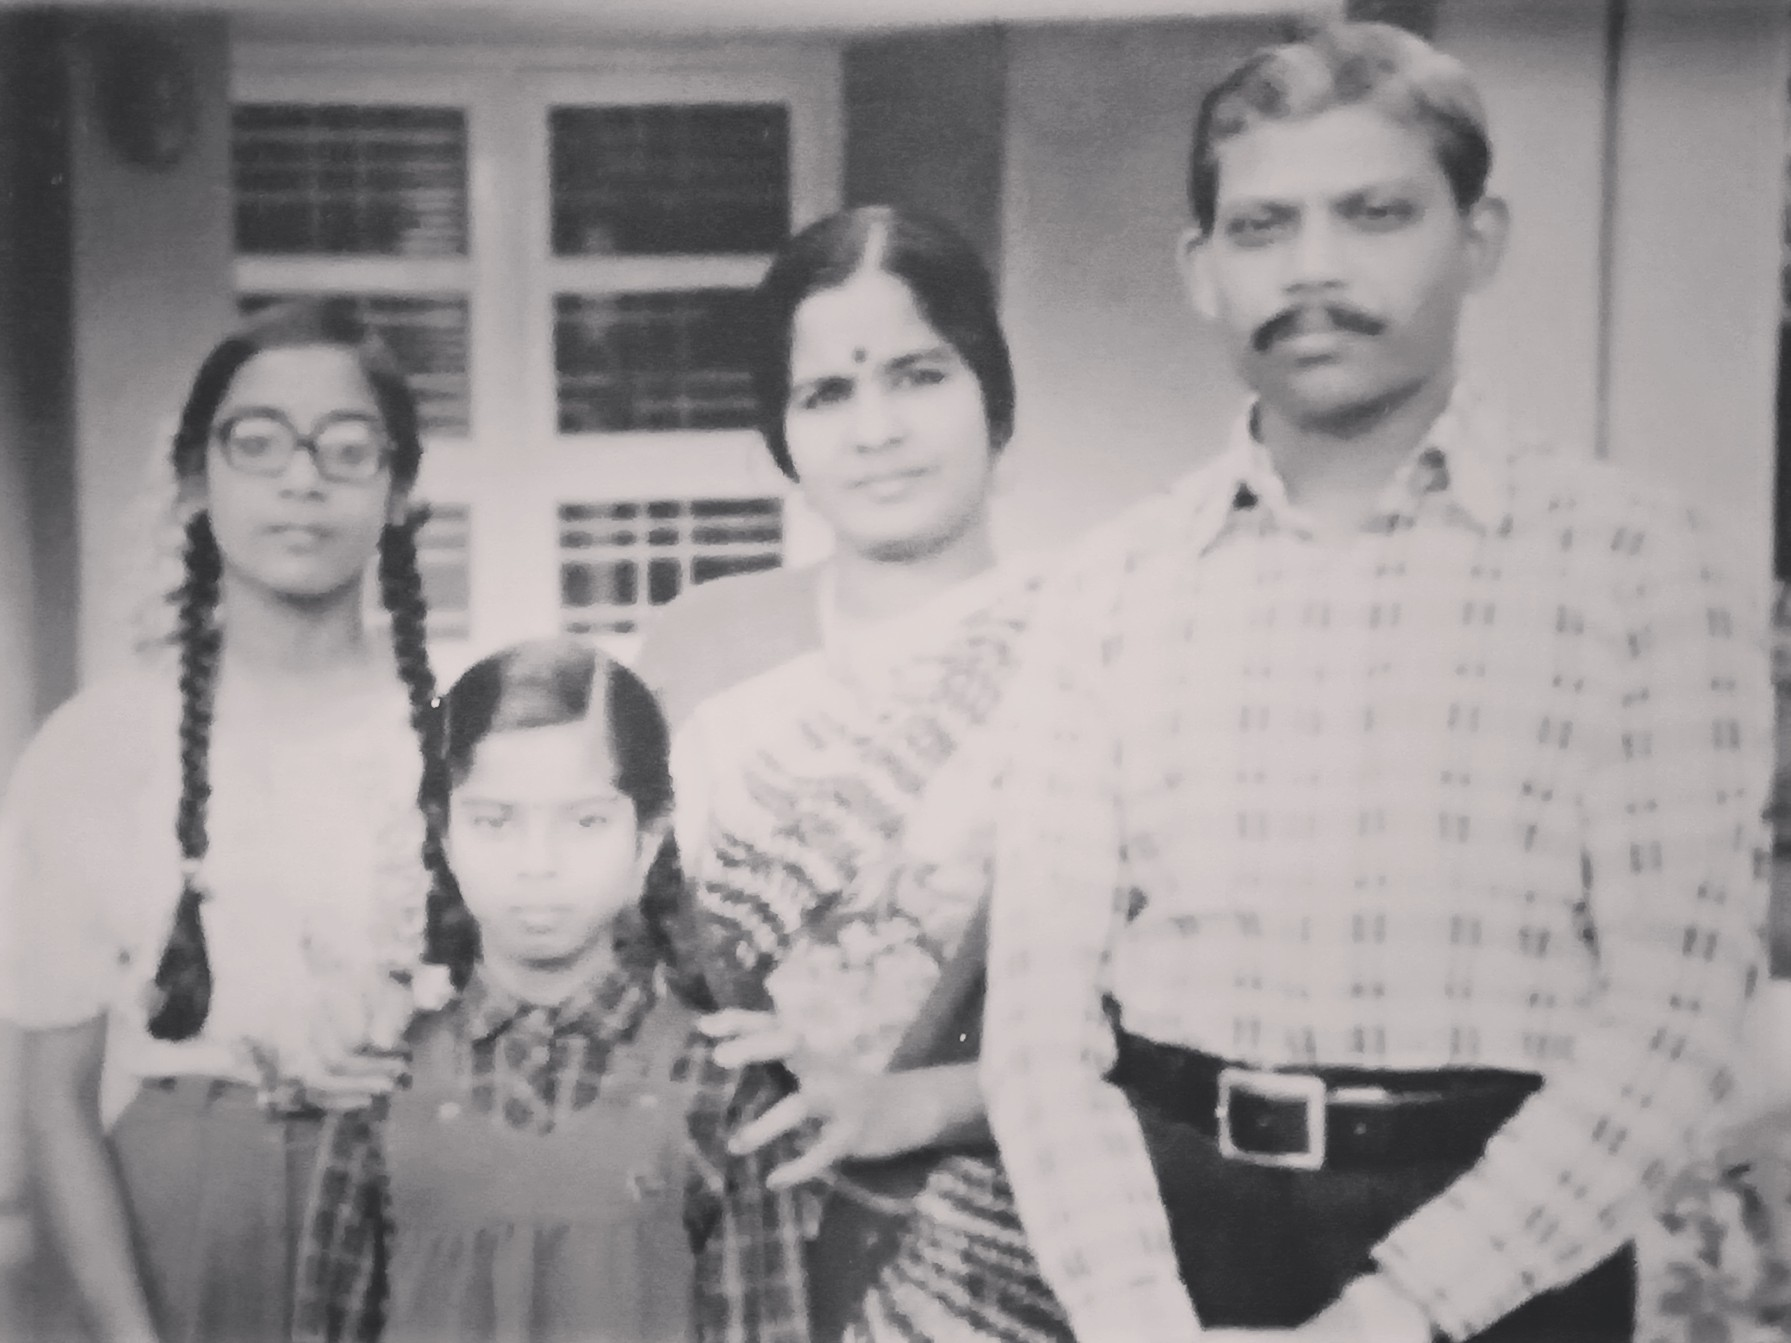
\includegraphics[width=0.8\textwidth]{images/Rajaji-03.jpg}
\caption{\small{Circa 1982, Poongodhai, Uma, Suthandra, GR.}}
\end{figure}

\vskip -10pt
Willis Lamb visited TIFR and gave many lectures on the recently 
discovered Mossbauer Effect. Biswarup Banerjee and myself took notes and 
brought out a TIFR report.
                 
I went on a trip to the Himalayas with KKG, Biswarup and Luiz Balazs. 
Balazs was a theoretical physicist visiting TIFR. We went to Katmandu 
and from there we trekked. Our destination was the Valley of Flowers and 
Gosainkund Lake, which was sacred to Lord Vishnu. That was at 14,000 
feet. After reaching 13,000 feet or so, we reached the snow-line and we 
could not climb further since we were not equipped for snow. Further we 
were told there were no shelters for the night. On previous nights we 
stayed in the huts of the villagers and finally in a cave. Beyond this 
point not even a cave would be there. The sherpa who accompanied us 
refused to go further. So we decided to turn back. But one of us, 
Balazs, refused. He said we cannot turn back without reaching our 
destination. In fact he was suffering from diarria and could not eat 
anything. He was the most frail among us. Still he was adamant and 
wanted to climb further. While we admired his courage and tenacity we 
did not want our trip to end in a tragedy. We forced him to return with 
us.

This Balazs is a tenacious character. He was well-known for his 
bootstrap calculations which was part of the S Matrix Theory. This 
theory was reigning over particle physics at that time. Udgaonkar and 
Virendra Singh were very much in it.

To begin with, I continued my research along lines connected to my PhD 
thesis research. I showed that the hadron Lambda (1405) cannot be a 
three-quark bound state, but it is a compo\-site of a baryon and meson, 
the so-called ``molecular hadron". I could construct a test for molecular 
hadrons. The test was simply that if it were a quark composite, the K 
matrix for meson-baryon scatte\-ring must have a pole but such a pole did 
not exist for K bar-N, pi-Sigma scattering. I talked about this result 
in two conferences, but did not publish in any journal.

I got into a controversy with my teacher Dalitz on the work on Lambda 
(1405), since earlier Dalitz, Wong and myself had wo\-rked on this hadron. 
Dalitz felt perhaps that he should be a coauthor in the K-pole paper. I 
wrote to him apologizing for what I did and explaining the circumstances 
in which this happened. Then I wrote a detailed paper making due 
references to Dalitz's work and also thanking him.

Much later after QCD came up, it was shown that QCD also supports the 
conclusion that Lambda (1405) is not a three-quark bound state.

Meanwhile Gell-Mann's current algebra was making prog\-ress and I worked 
on Current Algebra for a while with L K Pandit and Virendra Gupta.

In 1970, the HEP Conference was held in Kiev, Russia. I was one of the 
delegates chosen by TIFR. They got the visa and bought the ticket. They 
brought them to me along with a form to be signed by me. I was supposed 
to sign a bond to work in TIFR for a certain number of years because 
TIFR was financing my trip. I refused to sign. I told Udgaonkar who was 
the Chairman of the Theoretical Physics Section that under the 
circumstances I would not go for the Conference. They said it was a mere 
forma\-lity, but I said I was against signing any bond, on principle. They 
wanted to consult the Director, MGK Menon. He was out of town, but on 
return, instead of coming to TIFR, he stayed in the Tata House! So I did 
not go to Russia. Looking back, the whole thing appears to be silly 
since I did not have any intention of leaving TIFR and so the bond was 
only a formality. I have described this event only because this is the 
only time I fought with TIFR. Because of this fight, TIFR removed the 
requirement of the bond subsequently!
\smallskip

Maybe as a consequence of this fight, I undertook a pilg\-rimage. I 
visited the temples at Kanchipuram, Thiruvannamalai, Srirangam, 
Kumbakonam, Chidambaram, Madurai, Srivilliput\-hur, Thiruvananthapuram and 
Suseendram. This was the first time I visited them except Madurai. I was 
truly amazed at the cultural magnificence of Tamil Nadu.

\vspace{-.3cm}

\subsection*{Kolar events:}

\vspace{-.2cm}

One morning, my wife who was looking at the Times of India, exclaimed 
``Look, your friend KVL Sarma's name is in the front page!". I looked and 
found she had missed my name. The news item in the front page said G 
Rajasekaran and KVL Sarma have discovered a new particle. The Kolar 
experiments discovered some events that could not be explained. KVL 
Sarma and myself interpreted those events as due to a new particle. I 
also described this in an article in Physics News. TOI looked at only 
this popular science article and wrote the story. I was flabbergasted. 
There was no mention of the experimenters (that included MGK Menon). I 
contacted TOI and asked them to withdraw the story or at least correct 
it. They refused and said I can send a letter to the editor.

TOI could have verified the authenticity of their story by phoning TIFR. 
They didn't. This is the level of science repor\-ting!

Recently at IMSc, MVN Murthy and myself have interpreted the 40-year old 
Kolar events as due to Dark Matter particles.
\newpage

\section*{Gauge Theory}

\vspace{-.2cm}

I became aware of Yang-Mills (YM) theory by reading J J Sakurai's paper 
in Annals of Physics in 1959. That was the first paper in which YM was 
used in particle physics. Sakurai constructed a gauge theory of strong 
interactions. I continued to be intere\-sted in YM theory from that time. 
Veltman's lecture at Varena where he talked about the conserved weak 
current impressed me very much and I felt that weak interaction must be 
described by a YM theory. So, when Weinberg's paper on the SU(2)xU(1) 
electroweak theory came out in 1967 I had no doubt that was the correct 
theory. I read the papers of Goldstone, Higgs and Kibble.

In the subsequent two or three years, I lectured on these at various 
places including TIFR. In particular, in June 1971, I gave a series of 
lectures on the gauge theory of weak interactions including Yang-Mills 
theory, Faddeev-Popov ghosts, Higgs mecha\-nism, electroweak theory, GIM 
mechanism etc. It came out as a SINP report. This was the first 
connected account of what became known as the Standard Model, anywhere 
in the world! It even contained my conjecture that the massless YM gauge 
quantum cannot exist as a particle because of the incurable infra\-red 
divergences (an early suggestion of what became known later as infrared 
slavery and colour confinement).

Nevertheless I failed to make any substantial contribution in gauge 
theory. This was partly because I had to take care of my sick father 
whom I had tried the treatments in the hospitals at Bombay and then in 
Madras, but to no avail. He passed away in May 1973.

I must refer to the peculiar circumstances under which I gave the gauge 
theory lectures at Saha Institute of Nuclear Physics (SINP) referred 
to above. In 1971, the whole of East Pakistan was in turmoil. Many 
refugees poured into Calcutta. Whole Calcutta was under siege. That is 
the time I went to SINP. Trilochan Pradhan who was my host made special 
arrangements for me. The driver who picked me up at the railway station 
was instructed to take a different route and take me to a different 
guest house. I was escorted with high security to SINP where my lectures 
were given. All over the City there were agitations and police shoo\-ting. 
Situation called for action by India. Indira Gandhi acted with a firm 
hand and Bangla Desh was born.
  
I became aware of t'Hooft's proof of the renormalizability of the 
electroweak theory which came out after my SINP lectures. Then came the 
discovery of asymptotic freedom of YM theory by Gross, Wilczek and 
Politzer and the construction of SU(3) colour gauge theory by Gell-mann, 
Fritzche and Leutwyler to describe strong interactions.

Renormalizability of electroweak theory and asymptotic fre\-edom of YM 
theory are the two most important discoveries in Quantum Field Theory 
after the discovery of renormalizability of Quantum Electrodynamics in 
1947-49. I missed the boat in both, although I was well-placed with 
potential to contribute. I had already studied path integrals which 
t'Hooft used in his proof and was already giving lectures on Wilson's 
Renormalization Group and Callan-Symanzig equations which are the 
ingredients in the discovery of asymptotic freedom.

Although I missed the stage, I was sitting in the front row. I could 
catch their significance as soon as the discoveries came tumbling one 
after another! The years 1971-73 were truly exi\-ting years. It was the 
watershed in the development of High Ene\-rgy Physics.
  
Actually, until t'Hooft's proof, as far as I know, nobody except Joe 
Schechter in Syracuse University who added a U(1) to cancel the 
strangeness-changing neutral current and myself had taken Weinberg's 
theory seriously. Even after t'Hooft, only a few theorists took it 
seriously. Situation changed dramatically after the discovery of the 
weak neutral current interaction in the CERN experiment by Perkins and 
others in 1973.

In 1969, TIFR's theoretical physics summer school was at Nai\-nital. Some 
memorable events took place there. Both Geo\-ffrey Chew and Francis Low 
lectured. Chew lectured on S Matrix\break Theory. I asked him a question: 
Since S Matrix theory addressed only strong interactions, what happens 
to weak and electromagnetic interactions? Chew gazed at the distant 
Himalayan peaks visible through the window for a few minutes and simply 
continued his lecture.

Low lectured on the divergence problem of the Fermi theory of weak 
interaction and described all the methods proposed to deal with the 
problem. This was two years after Weinberg's paper. I asked Low at the 
end of his lectures why was he ignoring the Yang-Mills theory of weak 
interactions. He merely stared at me and refused to answer my question. 
He described seven or eight unnatural ways of solving the weak 
interaction problem but left out the one way that turned out to be the 
right way. To this day I have not understood how such a thing is 
possible, Low being a very experienced physicist. Somebody said it was 
because Low did not like Weinberg! Tapas Das and myself took notes of 
Low's lectures and brought it out as a TIFR yellow report.

\vspace{-.5cm}

\section*{Neutral Current}
\vspace{-.2cm}


Weak neutral current (NC) interaction is almost as strong as the usual 
charged current (CC) weak interaction but lay undisco\-vered all those 
years. It could have been discovered many years earlier if only the 
experimenters did not listen to some theorists who said NC cannot exist. 
The theorists thought that NC would lead to strangeness changing NC 
decays which were not seen, but they forgot that there could be 
strangeness non-changing NC. So the experimenters ignored some data which 
were actually due to NC. But the clinching experimental proof was 
possible only after the huge Gargamelle bubble chamber was constructed 
at CERN. Because of its size they could clearly distinguish a pion 
from muon and this was crucial for the discovery of NC through the 
absence of muon in neutrino collision.

\newpage
As soon as the discovery of NC was announced, KVL Sarma and myself 
produced the first model-independent analysis of de\-ep inelastic data. JJ 
Sakurai called our equations ``Master Equations". His analysis of elastic 
scattering coupled with LM Sehgal's of single pion production and our  
Master Equations led to the complete determination of NC coupling 
constants.


The evolution of the name starting from Gauge Theory is inte\-resting. As 
soon as t'Hooft showed the renormalizability of electroweak theory I 
calculated the radiative correction to muon decay and sent it to 
Physical Review for publication. I had put the title as ``Radiative 
correction to the muon decay in gauge theory". Physical Review changed 
it to ``Weinberg's gauge theory". In 1972 the HEP Conference was held at 
Chicago that I atten\-ded. That is where gauge theory was presented as a 
Rappor\-teur's talk for the first time. BW Lee gave the talk. He called 
the theory as ``Salam-Weinberg gauge theory". Salam and Gell-Mann were 
sitting in the first row and I happened to be sitting in the second row 
just behind Salam and Gell-Mann. As soon as Lee mentioned 
``Salam-Weinberg gauge theory", Gell-Mann gave a nudge to Salam with his 
elbow. Later when the Nobel Prize was given, Glashow's name was added 
and the theory beca\-me Glashow-Salam-Weinberg theory. This is certainly 
justi\-fied since Glashow was the first to discover that SU(2)xU(1) was 
the correct gauge group for electroweak theory and also he was one of 
the inventors of the Glashow-Iliopoulos-Maiani (GIM) mechanism to remove 
the strangeness changing neutral current. However I now prefer to call 
it the Electroweak Theory!

\vspace{-.4cm}

\section*{Integrally charged quarks}

\vspace{-.2cm}

There is the possibility of quarks having integral charges unlike the 
Gell-Mann - Zweig (GZ) quarks which are fractionally charged. The former 
were introduced by Han and Nambu (HN). Probir Roy and myself constructed 
a colour gauge theory based on HN quarks and we got two interesting 
results. Although HN quarks have inte\-gral charges, as observed in deep 
inelastic scattering they will appear as fractionally charged. Further 
in this theory gluons are electrically charged and hence they also 
contribute to deep inelastic scattering. We published this in Pramana 
and soon we saw a preprint by Pati and Salam who also had the same 
theory. Although they also obtained the correct theory, they missed the 
fact that gluons in this theory are charged and hence contribute to 
deep-inelastic scattering. We pointed this out to them. Immedi\-ately 
Salam sent us a cable saying they were wrong and we were right. They 
also corrected their paper, but they did not acknowledge us!

Subsequently, after I shifted to Madras, with my students and 
collaborators (T Jayaraman, Lakshmibala and Saurabh Rindani) I tested 
this theory by comparing the results with experi\-mental data on deep 
inelastic scattering and electron-positron collisions. The theory agreed 
with data and could not be ruled out.

To this day this theory of HN quarks has not been ruled out by 
experiment and may even be the correct theory. Colour is broken in this 
theory spontaneously.

\vspace{-.3cm}

\section*{Visit to Hawaii}

\vspace{-.2cm}

In 1974 my friend Sandip Pakvasa invited me to visit him at Ha\-waii 
University. Since I had two young children, I hesitated to undertake the 
travel. It was my friend C S Warke who said it would be a good 
opportunity for the family to see USA. I trave\-lled with my wife and 
children. Spent two very interesting mon\-ths in Hawaii and worked with 
Sandip. In October 1974, the earth-shaking news came. That came to be 
known as the psi particle later. At that time we only knew that some 
extraordinarily narrow peak had been seen in electron- postitron 
collisions. It was as if anthropologists stumbled upon a group of humans 
in some remote corner of the world who lived for 100,000 years! After 
that there was no peace! San Fu Tuan was constantly at the phone trying 
to get more information on the narrow peak from Stanford and other 
Centres. He, Sandip and me wrote up some dozen interpretations for the 
narrow peak and published it. This is one of the earliest papers on the 
subject. Fortunately we did include the one correct interpretation 
namely the psi particle was a bound state of a charmed quark and the 
corresponding antiquark.

After Hawaii, I took my family on a tour of mainland USA visiting UCLA, 
University of Texas at Austin, Rochester University, City College of New 
York, Maryland University and Syracuse University. In all these places I 
gave seminars.

\section*{How we proved three Nobel Laureates wrong!}

\begin{enumerate}
\itemsep=0pt
\item By discovering the ``shadow poles" Dalitz and myself pro\-ved CN Yang 
wrong.
\item By working out the Han-Nambu model correctly, Probir Roy and myself 
pointed out the error of Abdus Salam and Jogesh Pati.
\item After I returned to TIFR in 1964, the discovery of CP vio\-lation by 
Cronin and Fitch excited the particle physics wo\-rld. During his visit in 
Caltech, Virendra Gupta (VG) published a paper in Physical Review 
Letters in which he had constructed what looked like an elegant model 
for CP violation. After his return to TIFR he discussed this with me and 
I discovered that his model violated CPT theorem and hence is not 
tenable. This was the shortest paper I ever published. Since in his 
paper VG had thanked Gell-Mann for discussions, he is the third Nobel 
Laureate I proved wrong!
\end{enumerate}

I have to balance the above by the following.
\newpage
\section*{My failed attempts}

\begin{enumerate}
\itemsep=0pt
\item This was soon after I joined TIFR in 1958. In the primordial nuclear 
synthesis there was a gap. In the successive cooking of nuclei starting 
from proton by absorption of a neutron, there seemed to be a gap at A = 
5 because $He^5$ is not bound. When I learnt that the hyper-nucleus 
Lambda-$He^5$ is bound, I thought that is the solution. I discussed it 
with Udgaonkar, but it did not work.
\item After CP violation was discovered from K decays into two pions in 
1964, I thought the ugly CP violation can be avoi\-ded by recognizing that 
since pions are quark-antiquark bound states, Bose statistics for pions 
is only approxima\-tely valid and without Bose statistics, CP violation 
cannot be concluded. This idea too did not work.
\item During 1964-64, with Arvind Kumar who joined me as a student, we 
undertook a massive calculation aiming to co\-nstruct a complete theory of 
hypernuclei. In fact Arvind Kumar managed to do an enormous amount of 
calculation. It did not lead anywhere.
\item I tried to generate the nucleon-pion coupling using the quarks of 
which N and pi were made. This also did not lead anywhere.
\item For quite a long time, I imagined quarks to be leptons. That would have 
been the natural explanation for quarks and leptons satisfying the same 
current algebra. I tried to construct a mechanism by which the weakly 
interacting leptons could sometimes exhibit strong interactions, but I 
failed.
\item During 1967-70, I tried to construct strong interactions fr\-om weak 
interactions. by using the divergences of Fermi's weak interaction 
theory. TD Lee had shown how the qua\-dratic divergences could be turned 
to strong interactions. Gell-Mann, Goldberger, Kroll and Ruderman wrote 
a nice paper showing how the quadratic divergences generate the diagonal 
(that is, the parity conserving strangeness conserving) sector that 
could be identified as the strong interactions. My aim was to redo these 
calculations usi\-ng the YM theory of weak interactions of Weinberg's 1967 
paper. But alas! t'Hooft proved the renormalizability of Weinberg's 
theory.

\vspace{-.4cm}

\end{enumerate}

\vspace{-.3cm}

%~ \vspace{-\topsep}
\section*{University of Madras (1976 to 1984)}

\vspace{-.2cm}


%~ \vskip -10pt
Everything was going very well at Bombay. So why did I decide to leave 
Bombay? There are several reasons. For some time Shiva Sena was gaining 
ground. When there was water shortage, they even wanted to send back all 
Madarasis. One day there was a big agitation in the streets. When I was 
waiting at Gymkhana for the TIFR bus, some goons got hold of one of my 
TIFR colleagues and beat him up. So I decided that when a chance came I 
must leave Bombay. Second reason was that my children hardly knew Tamil 
and my wife spoke only Tamil. So I felt that my children must grow up in 
Tamil Nadu. A third reason was that I felt I must use my knowledge to 
teach at a University. Those were the days when Indira Gandhi introduced 
the slogan ``Science for the People". B M Udgaonkar was advising that 
TIFR people must go to the universities to teach. But none of these is a 
strong reason. So I must attribute my shifting to Madras to fate!

First I was selected as a Professor at the Guindy Engineering College by 
VC Kulandaiswamy who was the Director of Technical Education at that 
time. Although the College was to be upgraded as the core of the Anna 
University to be formed, I felt it was not the proper job for a 
physicist.

I got a second chance when Madras University advertised for a 
Professorship in the Dept of Theoretical Physics. I applied and got the 
job even without an interview. But there were many difficulties. For one 
thing although the offer matched my basic salary, my total remuneration 
at the University was conside\-rably lower than that at TIFR since at TIFR 
I was getting a large Dearness Allowance (DA) which was not available at 
the University. Malcolm Adiseshaiah increased the salary considerably to 
match my salary plus DA at TIFR. I decided to accept the offer and 
joined Madras University in July 1976.

At TIFR I was living at the comfortable quarters provided by the 
Institute. At Madras I was literally thrown to the streets. I had to 
change the rented apartment three times until I finally managed to buy a 
old house.

A comparison between TIFR and Madras University would be apt at this 
point. I had figures to show that at TIFR, for eve\-ry thousand rupees 
spent on salary for an academic person, ten times that much was spent on 
infrastructure, including library, money for attending conferences etc. 
In this I am not inclu\-ding the comfortable living quarters that TIFR 
provided. At the University, absolutely nothing beyond the bare salary.

Here I must mention my friend V Radhakrishnan who helped me on many 
occasions. But for him I would not have survived in Madras. He was a few 
years senior to me and I knew him and his wife Kaveri even at Bombay. He 
was a student of KK Gupta.

At Bombay, many were the evenings when he used to take me to Chembur, 
Sion or Matunga to listen to heavenly Carnatic Music by Chembai 
Vaidhyanatha Bhagavathar, Ariyakkudi, Semmangudi, MD Ramanathan or the 
celestial MS Subbulakshmi.

At the Dept of Theoretical Physics, there was PM Mathews who was the 
Head and G Bhamathi, M Seetharaman, MD Srinivas and SS Vasan were the 
faculty members. Malcolm Adise\-shaiah introduced many rapid changes. He 
introduced MSc teaching at the Departments. Until then MSc was done only 
at the Colleges. The starting of MSc coincided with my joining. There 
were many good students. He introduced the semester system, monthly 
meetings of all professors with the VC and rotation of the headship of 
the departments. Since I was the seniormost after Mathews, I had to take 
up the headship.

There was V Srinivasan who joined as a visiting member. He was a 
remarkable person. He became a good friend of mine and we worked 
together on many papers. I took SD Rindani as a new faculty member and 
JK Bajaj and V Sriram as post-docs under my UGC project ``Gauge Theory". 
T Jayaraman first and then La\-kshmi bala who were MSc students became my 
PhD students. So we had a very active group.

During my stay in the University, the Department of Theore\-tical Physics 
was the venue for two activities. Bajaj wrote many papers on Grand 
Unification but got frustrated that the scale of that theory was far 
away from presently accessible energies. So he left Physics. Along with 
MD Srinivas and MS Sriram he founded a movement called Patriotic 
People-oriented Science and Technology (PPST) whose main theme was that 
unless we pay attention to Science and Technology done in India from 
anci\-ent times, science will not take root in this country. They brou\-ght 
out a journal named PPST. The journal does not exist any more. But the 
three of them founded the Centre for Policy Stu\-dies at Chennai and 
another institution in Delhi.

The Department= proved to be the venue where Sriram cour\-ted Lakshmibala 
and married her!
\vskip 1pt
One morning an official car came to my residence to pick me up. It was 
because of a case against the University. I had condu\-cted a meeting of a 
selection committee for a research assistant's post and made the 
selection. The former occupant of that post went to the court claiming 
he should have been selected. So the University sent me to meet the 
advocate of the University. That was P Chidambaram who later on became a 
Central Minister. Chidambaram asked me whether the person was selected 
by a regular selection committee on the basis of the academic 
qualifications of the candidate. I said ``Yes" and he asked me to sign 
that as a written statement. I did so. Chidambaram said ``Profe\-ssor, I 
will now take care of it." That was that. The court decided in the 
University's favour.

Two bright students from IIT, Kanpur wrote to me saying they wanted to 
join me as research students. One was Avinash Dhar and the other was 
Ramadass. I think they were advised by my friends HS Mani and R 
Ramachandran, both at IITK. Avinash came. The University did not have 
any research fellowship mo\-ney and no hostel facility. Avinash used his 
own money and managed to stay somewhere. He survived for a few weeks 
this way. Meanwhile he got admission into TIFR graduate school and I 
advised him to go. Because of this experience, when Ramadass wrote to 
me, I told him to go to TIFR. Both of them are now senior academicians 
at reputed institutions.

Malcolm decided to quit in 1979 and the University plunged back into its 
original state. All the measures that Malcolm introduced were undone one 
by one. MSc was stopped. I was getting frustrated.

\vspace{-.4cm}

\section*{Japan (1980 and 1981)}

\vspace{-.2cm}

Advised by my friend Sandip Pakvasa, Hirotaka Sugawara of KEK Japan 
invited me. I went and spent two years (1980 and 81) there. KEK is the 
National Laboratory for High Energy Physics of Japan. Apart from 
Sugawara there were many other bright theorists such as Yoshimura and 
Kobayashi. I interacted with the experi\-mental groups too. Yasumi, an 
experimental nuclear physicist who wanted to measure the mass of the 
antineutrino in the internal bremsstrahlung electron capture of Holmium 
asked me to join him as a theorist. I calculated the rate of this 
process. This was my only experimental paper.


I must say something about the Japanese physicists and students whom I 
encountered. Their dedication and capacity for hard work were 
incredible. Even physicists in their sixties and seventies used to work 
in their rooms or laboratories very late into the night.


I had taken my family of wife and two daughters to Japan, but sent them 
back during my second year so that the school education of Poongodhai, my 
elder daughter was not affected too much. While in Japan both my 
daughters went to a Japanese school and picked up considerable Japanese.


I had many friends in Japan. Among them I must mention Roger 
Bissionnette who was an engineer in accelerator science. We used to 
travel together in Japan during my second year there.


In Japan I learnt three things: car-driving, Karate and Japa\-nese 
language. Although I learnt to drive a car, I could not under\-go the 
driving test since that required considerable knowledge of Japanese 
language. So I was driving only within the KEK campus! While learning 
Japanese, I found many remarkable similari\-ties between it and Tamil. Of 
course all these three things that I learnt in Japan, quickly evaporated 
after return to India!


While I was at KEK, a memorial meeting for Tomonaga (who had passed away 
recently) was going to be held at Kyoto. All of us in the Theory group 
went to attend that. Schwinger was going to give the memorial speech. 
The announced title was ``The two shakers of Physics". I thought the two 
shakers were Relati\-vity and Quantum Mechanics. Schwinger pointed out 
that his Germani\-c name ``Schwinger" meant ``shaker" and ``Shin" in the name 
of Shin Itiro Tomonaga also meant ``to shake". So those are the two 
shakers! He gave an excellent speech telling us how Schwinger and 
Tomonaga developed QED sitting on either side of the Pacific, unknown to 
each other. It was war time and there was no communication. The parallel 
went further. Schwinger described how both independently developed the 
theory of wave guides and microwave cavities needed in war. Although the 
trip\-let Tomonaga, Schwinger and Feynman were involved in deve\-loping QED, 
Schwinger hardly mentioned Feynman. The only mention of Feynman was that 
Feynman missed the correct numerical factor in one of the higher order 
calculations!
\vskip 1pt
I returned to Madras University in 1982 and was not happy. I felt sad 
that a lot of progress was taking place in High Energy Physics and I was 
stuck in this hole.

In 1982 I visited ICTP, Trieste. It happened that the W and Z bosons 
were discovered at CERN at that time. My friend Sandip Pakvasa informed 
me about the W discovery and I had the good fortune to convey that 
information to Abdus Salam when I met him. He was very happy and thanked 
me. All the time he was munching groundnuts!

At the ICTP canteen a few of us including a Pakistani physicist were 
discussing things and I mentioned the following. I said that Salam is 
the only scientist who could be the Director of an Institution and at 
the same time made top-class discoveries. He discovered Superspace. I 
also said in a comparable situation Ho\-mi Bhabha had to abandon his 
research while managing TIFR and DAE. Immediately the Pakistani 
physicist said that is possible only if you can manage two wives!

\vspace{-.3cm}

\section*{Some interesting events}

\vspace{-.2cm}

In 1963 I left Chicago for New York to take the ship for England. I 
wanted to visit my friend SV Rangaswamy at Philadelphia. At the New York 
bus station I was supposed to take the bus for Philadelphia. From inside 
the station I could see the bus about to start. I dashed for it, but was 
stopped with a loud crash. I had crashed into a glass wall. Immediately 
security men took care of me. My face and body were covered with broken 
glasses. The doctors attended on me and carefully removed the glass 
pieces from my eyes. They also treated the minor cuts. I was very much 
worried that I may have to pay for damaging the glass walls. I was told 
that it was the opposite; I can claim for the shock and injuries that I 
suffered. The glass wall did not have any lettering or other warning 
sign and so the bus station was liable to pay. But I did not want to 
make any claim. The security guards were with me and put me in the 
correct bus.

During my trip to USA in 1974 with my family we visited many 
Universities as I already described. I had bought air ticke\-ts for the 
whole trip involving New York, Hawaii, Los Angeles, Austin, Maryland, 
Syracuse and Rochester. At the Syracuse airport, at the check-in counter 
I was told that my ticket was not valid. We went on arguing, but the 
official did not allow us to board. Meanwhile my luggage was already put 
in the aircraft. I lost patience and shouted at the officials. I threw a 
tantrum that frightened everybody. But it worked. Since the plane had 
already left for Rochester, they put us in a tiny fore-seater plane. We 
reached Rochester and saw that our luggage was already wai\-ting there.


When I was in Bombay, I traveled with Virendra Singh to attend the 
Conference on Few Body Problems organized by AN Mitra of Delhi 
University. We reached the airport very early in the morning. After 
checking in, we sat in the departure lounge and began our conversations. 
Our discussion was perhaps very interesting. We lost the sense of time 
and did not notice that departure of our plane was announced. After a 
while we noticed\- that we were the only two passengers sitting there. We 
saw through the glass door that our plane was in the runway. We ran past 
the security guards and when we were near the plane, the pilot saw us 
and began to move the plane. We ran after the taxiing plane. The 
security guards took us inside the airport.


We complained that we missed the plane since the annou\-ncements were not 
audible ignoring the fact that they were audible to the other 
passengers! Finally they found two seats in the next plane, but we had 
to buy them. Fortunately V Singh had his cheque book. At Delhi, we 
missed only the morning session.


After returning to Bombay, we wrote to Indian Airlines as\-king for the 
refund of the fare that we had paid for the missed flight. There was no 
response. In spite of our repeated appeals, Indian Airlines refused to 
pay. We then had a bright idea. We had used the official letterhead of 
TIFR. This time we sent a copy of that letter to JRD Tata, the Chairman 
of the Governing Council of TIFR and also the boss of Indian Airlines. 
In a few days, we got our money!

\newpage

I lived in the TIFR quarters at Chembur during 1967 to 1970 and commuted 
for four years. The quality of construction of the flat where we stayed 
was very bad. One day a big piece of the ceiling fell on the bed very 
near the place where my three-year old daughter Poongodai was sleeping. 
I met Bhandarkar the Administrative Officer at TIFR and demanded that I 
be allowed to occupy the Colaba quarters which were almost ready. He was 
making some excuses for the delay and I shouted at him right and left. 
This happened in the fourth floor of TIFR. He was a tall well-built man, 
but he simply ran for life, unable to bear my onslaught. I chased him 
until he disappeared into one of the rooms at the end.

It seems I was quite a terror those days!

As a consequence of this event, I was allowed to occupy the new flat in 
Colaba. I was the first occupant with many facilities not quite on. For 
instance the lift will close after we are in and take us to the basement 
where the door would not open. But that is another story.

Since both my daughters lived in the USA, every year we visi\-ted them. 
Once the immigration officer at Los Angeles airport saw that I had an 
invitation to visit the University of California at Riverside. He turned 
to me and said, ``Since you are a Professor of Physics, I want to ask you 
a question. Is Einstein the greater scientist or Hawking?" I 
said, ``Without question, Einstein!" He did not agree and we went on 
arguing for a while. Meanwhile he stamped my passport and I came out. 
Only when my daughter saw the passport, we realized the mistake. In my 
enthusiasm of argument I was not attentive and the officer stamped B2 
visa. He was supposed to give B1, otherwise I cannot be paid by the 
University. My daughter Uma said it can be changed at the immi\-gration 
office.

Early morning next day, Uma drove me for an hour from Redlands to the 
Los Angeles immigration office where the line was long even that early. 
There were many Mexican immigrants whose entry is through Los Angeles. 
When my turn came, I told the officer about my problem. He said once the 
immigration offi\-cer at the port of entry stamps it, not even the 
President of United States can change it. I will have to go out of the 
country and while reentering I can change it.

Uma wanted to take me to the border town Tijuvana near San Diago. I was 
supposed to walk down and cross the border into Mexico and reenter. I 
vetoed the idea.

As an anticlimax, the secretary in the Physics Department paid me the 
money without looking at what was stamped in the passport.

